\documentclass[12pt]{article}
\usepackage[margin=1in]{geometry} 
\usepackage{amsmath,amsthm,amssymb,amsfonts}
%\usepackage{xcolor}
\usepackage{graphicx,fancyhdr,algorithm,algorithmic}
\usepackage[space]{grffile}
\usepackage{titlesec}
\usepackage{multicol}
\usepackage{enumitem} 
\usepackage{tikz}
\usepackage{tikz-qtree}
\usetikzlibrary{arrows,automata}


\cfoot{\thepage}
\renewcommand{\headrulewidth}{0.4pt}
\renewcommand{\headwidth}{\textwidth}
\renewcommand{\footrulewidth}{0.4pt}

%some custom commands for problem 2
%want some nice colors
\definecolor{darkred}{rgb}{.87,0,0}
\definecolor{niceblue}{rgb}{.392,.584,.929}
%change the font, change the color, and raise the first word's letters slightly
\newcommand{\firstword}[1]{\textsf{{\color{darkred}{\raisebox{.3em}{#1}}}}}
\newcommand{\secondword}[1]{\textsf{{\color{niceblue}{#1}}}}


\theoremstyle{definition}
\newtheorem{problem}{Problem}
\newtheorem{claim}{Claim}
\newtheorem{definition}{Definition}
\newtheorem{theorem}{Theorem}
\newtheorem{lemma}{Lemma}
\newtheorem{observation}{Observation}
\newtheorem{question}{Problem}

\newenvironment{solution}{\bigskip\noindent{\it Solution.}  \ignorespaces}{\hfill\qed}

\usepackage{hyperref}
\hypersetup{
    colorlinks=true,
    linkcolor=blue,
    filecolor=magenta,      
    urlcolor=cyan,
}
\urlstyle{same}
\PassOptionsToPackage{hyphens}{url}


\newcommand{\homework}[6]{
   \pagestyle{myheadings}
   \thispagestyle{plain}
   \newpage
   \setcounter{page}{1}
   \noindent
   \begin{center}
   \framebox{
      \vbox{\vspace{2mm}
    \hbox to 6.28in { {\bf CS256:~Algorithm Design and Analysis \hfill #1} }
       \vspace{6mm}
       \hbox to 6.28in { {\Large \hfill #2 \normalsize{(#3)}  \hfill} }
       \vspace{6mm}
     \hbox to 6.28in { {\it Instructor: #4 \hfill  Solution template: #5} }
   }
   }
   \end{center}
   \markboth{#1}{#1}
   \vspace*{4mm}
}

\begin{document}
\homework{Spring 2021}{Assignment 5}{due 03/30/2021 }{Shikha Singh}{\href{https://www.overleaf.com/read/kscdpffcmmrd}{\em Overleaf}}

\noindent
{\bf Note.} This assignment is due a day early than usual:  it is due on Tuesday March 30.\\

\noindent
For full credit when describing a dynamic programming algorithm, you must clearly state the following parts:

\begin{enumerate}[ leftmargin=*, label = (\alph*)]

\item {\bf Subproblem definition:}  your subproblem must have an optimal substructure. 

\item {\bf Recurrence:}  how should the next subproblem be computed using the previous ones? This is the core of your algorithm and its correctness.\footnote{A less ideal alternative to a recurrence: clear pseudocode of the iterative DP algorithm.}   
You must {\bf explain in words} how you arrived at the particular recurrence.

\item {\bf Base case(s):}  you need to start somewhere!  

\item {\bf Final output:}  in terms of your subproblem.

\item {\bf Memoization data structure:}  this may often be obvious but should not be skipped.

\item {\bf Evaluation order:}  describes the dependencies between the subproblems.

\item {\bf Time and space analysis}  
\end{enumerate}

For this assignment, the above pieces are sufficient to justify your solution---that is, {\bf you do not need to formally prove correctness via induction}.
The first problem is solved to give you a template of how to organize your solutions.


\bigskip

The problems in this assignment are in (approximate) order of difficulty and you are encouraged to attempt
them in that order.   





\newpage

\begin{question}(Erickson 3.3) Suppose you are given an array $A[1,\ldots, n]$ of numbers, which may be positive,
negative, or zero, and which are not necessarily integers. 

Describe and analyze an algorithm that finds the largest sum of elements
in a contiguous subarray $A[i \ldots j]$. So if the array consists of only positive numbers, then the largest sum of contiguous elements would just be the sum of all the elements.   
If the array is only made up of negative numbers, then the largest subarray is made up of the smallest such number.  (To simplify things, we are not allowing empty subarrays).

As an example consider an array $A = [-6, 12, -7, 0, 14, -7, 5]$, then the contiguous subarray with the largest sum is $[12, -7, 0, 14]$ with the sum of $19$.
If the subarray is $B=[-4, -1]$, then the contiguous subarray with the largest sum is $[-1]$ with the sum of $-1$.



\textbf{Note.} This problem has been a standard computer science interview question
since at least the mid-1980s and can be solved via a variety of approaches.  We will use a dynamic-programming approach for this question.  
\end{question}


\begin{solution}
This dynamic programming problem is similar to the longest increasing subsequence problem we discussed in class.

\begin{itemize}
    \item {\bf Subproblem definition:} Let $M(i)$ denote the optimal (largest) subarray sum ending at index $i$ of the array (and including $A[i]$).
    
    \item {\bf Recurrence:}  Let us think of an element $A[j]$, either $A[j]$ extends a contiguous subarray ending at $A[j-1]$ or it does not and starts its own singleton subarray.  Taking the maximum value of the two cases gives us the largest subarray sum ending at index $j$.  
    
    Thus, we get the following recurrence for $M(j)$:
    
    \[M(j) = \max\{M(j-1) + A[j], A[j]\}\]
    
    \item {\bf Base case:} $M(0) = 0$ or $M(1) = A[1]$.

    \item {\bf Final solution:} given by taking the maximum over all the $M(j)$'s that is, $\max_{1 \leq j \leq n} M(j)$.
    
    
    
    \item {\bf Memoization structure:}  We can store the values of $M[0, 1, \ldots, n]$ in a linear size array. (We can actually do a lot better, we can just keep $O(1)$ state since we only need $M(j-1)$ while evaluating $M(j)$, not the previous values, and need to maintain a maximum-so-far for the final solution.  Just a clever space optimization).  
    \item {\bf Evaluation order:} the evaluation of the dynamic program proceeds left to right, starting from $j = 1$ and going up to $j = n$.
    
    \item {\bf Time and space analysis:}  To evaluate $M(j)$ takes $O(1)$ time for each $j$.  To compute the final solution, we need to take a maximum over these values, which can be done in $O(n)$ with a linear scan afterwards or done with $O(1)$ time per step of the dynamic programming evaluation.  Thus, the overall running time is linear.  The space usage is linear if you store $M(j)$'s or constant if you don't remember the $M(j)$ values.  
\end{itemize}
\end{solution}



\newpage
\begin{question}(Kleinberg Tardos 6.1) 
Let $G = (V, E)$ be an undirected graph with $n$ nodes. A subset of the nodes is called an \emph{independent set} if no two of them are joined by an edge. Finding large independent sets is difficult in general; but here we'll see that it can be done efficiently if the graph is simple enough.
	
Call a graph $G =(V, E)$ a path if its nodes can be written as $v_{1}, v_{2}, . . . , v_{n}$, with an edge between $v_{i}$ and $v_{i+1}$, for $i \in \{1, 2, \ldots, n-1\}$. With each node $v_{i}$, we associate a positive integer weight $w_{i}$. The problem we want to solve is the following: Find an independent set in a path $G$ whose total weight is as large as possible.


For example, consider the path in Figure~\ref{fig:path}, the maximum weight of an independent set is $14$.

%latex can do for loops and (albeit annoyingly) some math!
%this can help make drawing figures a little easier
\begin{figure}[h]
    \centering
    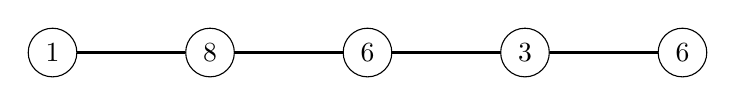
\begin{tikzpicture}
      %this draws the nodes
      \node [style={circle,draw}] (0) at (2,0) {1};
      \node [style={circle,draw}] (1) at (4,0) {8};
      \node [style={circle,draw}] (2) at (6,0) {6};
      \node [style={circle,draw}] (3) at (8,0) {3};
      \node [style={circle,draw}] (4) at (10,0) {6};
      %this draws the lines
      \foreach \x in {0,...,3}
        \pgfmathtruncatemacro{\nextnode}{\x + 1}
        \draw[thick] (\x) to (\nextnode) ;
    \end{tikzpicture}\caption{The maximum weight of an independent set is $14$ in this example.}\label{fig:path}
  \end{figure}
  



\begin{enumerate}[label = (\alph*)]
  \item Give a counterexample to show that the following ``pick the heaviest weight'' greedy algorithm does not always work.  You should say what the greedy algorithm returns,
   and what the correct answer is.

    \begin{itemize}[noitemsep, nolistsep]
      \item Start with $S = \emptyset$
      \item While some node remains in $G$
        \begin{itemize}
          \item Pick a node $v_i$ of maximum weight and $v_i$ to $S$
          \item Delete $v_i$ and its neighbors from $G$
        \end{itemize}
      \item Return $S$
    \end{itemize}

  \begin{solution}

  \end{solution}





  \item Give a dynamic-programming algorithm that takes an $n$-node path $G$ with weights and returns the {\em value} of the independent set of maximum total weight.  
\end{enumerate}
\end{question} 

\begin{solution}

\end{solution}

 

\begin{solution}
    
    \begin{itemize}
        \item {\bf Subproblem:} % give a clear definition of the DP subproblem
        
        \item {\bf Recurrence:} 
        % you should also explain how you constructed the recurrence in words 
        
       \item {\bf Final solution:} % in terms of the recurrence
        
        \item {\bf Base case(s):} % where should we start 
        
        \item {\bf Memoization structure:} % may be straightforward but need to include
        
        \item {\bf Evaluation order:} 
        
        \item {\bf Time and space analysis:}
        \end{itemize}
\end{solution}


\newpage
\begin{question}(Kleinberg Tardos 6.3) Let $G = (V, E)$ be a directed acyclic graph where the topological ordering
of nodes is $v_1, \ldots, v_n$.  A  reminder that a topological ordering of a DAG has the following property: {\em each edge goes from a node with a lower index to a node with a higher index. That is, every directed
edge has the form $v_i, v_j$ with $i < j$.}  Thus, the source node $v_1$ has no incoming edges.
 
We further assume that in graph $G$ each node except $v_n$ has at least one outgoing edge.
See Figure~\ref{fig:2} for an example.



Given $G$ and its topological ordering, we want to find the {\em length} of the longest path that begins
at $v_1$ and ends at $v_n$.  (The length of a path is the number of edges in it.)

\begin{figure}[h]
\centering
	\includegraphics[width=.7\linewidth]{dag.png}
	\caption{The correct answer for this ordered graph is 3: 
the longest path from $v_1$ to $v_n$ uses the three edges $(v_1, v_2),(v_2, v_4)$, and $(v_4, v_5)$.}\label{fig:2}
\end{figure}

\begin{enumerate}[label=(\alph*)]

\item Show that the following algorithm does not correctly solve this problem, by giving a counterexample. In your
example, you should say what the correct answer is and what the above algorithm finds.

    \begin{itemize}[noitemsep, nolistsep]
      \item Set $w = v_1$ and $L =0$ 
      \item While there is an edge out of node $w$:
        \begin{itemize}
          \item Choose the edge $(w, v_j)$ for which $j$ is as small as possible 
          \item Set $w = v_j$ and increment $L$ by $1$
        \end{itemize}
      \item Return $L$ as the length of the longest path 
    \end{itemize}


\begin{solution}
% you can uncomment the below code if you want to include example.png in your PDF
%\begin{figure}[h]
%\centering
%	\includegraphics[width=.6\linewidth]{example.png}
%	\label{fig:2a}\caption{Counter-example for part 2a.}
%\end{figure}
\end{solution}

\item Give an efficient dynamic programming algorithm that returns the {\em length} of the longest path that
begins at $v_1$ and ends at $v_n$.

\end{enumerate}
\end{question}

\begin{solution}
    
    \begin{itemize}
        \item {\bf Subproblem:} % give a clear definition of the DP subproblem
        
        \item {\bf Recurrence:} 
        % you should also explain how you constructed the recurrence in words 
        
       \item {\bf Final solution:} % in terms of the recurrence
        
        \item {\bf Base case(s):} % where should we start 
        
        \item {\bf Memoization structure:} % may be straightforward but need to include
        
        \item {\bf Evaluation order:} 
        
        \item {\bf Time and space analysis:}
    \end{itemize}
\end{solution}





\newpage
\begin{question}(Erickson 3.6)

  A shuffle of two strings  $X$ and  $Y$ is formed by interspersing the characters into a new string, keeping the characters of  $X$and  $Y$in the same order.For example, the string \textsf{BANANAANANAS} is a shuffle of the strings \textsf{\color{darkred} BANANA} and \textsf{\color{niceblue} ANANAS} in several different ways. 

  \bigskip

  %here's some latex for you!
  %the commands \firstword and \secondword are homemade commands, defined at the top
  %of the document.  The percent signs % are comments---but here they're used at the end
  %of the line to comment out the invisible "nextline" at the end of the line---much of the following
  % is on the same line.
  %\hspace{\fill} balances horizontal space---think of it as "pushing out" with equal force on either side
  \hspace{\fill}~
  \firstword{BANANA}\secondword{ANANAS}~
  \hspace{\fill}~
  \firstword{BAN}%
  \secondword{ANA}%
  \firstword{ANA}%
  \secondword{NAS}~
  \hspace{\fill}~
  \firstword{B}%
  \secondword{AN}%
  \firstword{AN}%
  \secondword{A}%
  \firstword{A}%
  \secondword{NA}%
  \firstword{NA}%
  \secondword{S}~
  \hspace{\fill}

  \bigskip

  Similarly, the strings \textsf{PRODGYRNAMAMMIINCG} and \textsf{DYPRONGARMAMMICING} are both shuffles of \textsf{\color{niceblue} DYNAMIC} and \textsf{\color{darkred} PROGRAMMING}:

  \bigskip
  \hspace{\fill}
  \firstword{PRO}%
  \secondword{D}%
  \firstword{G}%
  \secondword{Y}%
  \firstword{R}%
  \secondword{NAM}%
  \firstword{AMMI}%
  \secondword{I}%
  \firstword{N}%
  \secondword{C}%
  \firstword{G}
  \hspace{\fill}
  \secondword{DY}%
  \firstword{PRO}%
  \secondword{N}%
  \firstword{G}%
  \secondword{A}%
  \firstword{R}%
  \secondword{M}%
  \firstword{AMM}%
  \secondword{IC}%
  \firstword{ING}~
  \hspace{\fill}
  \bigskip



  \begin{enumerate}[label = (\alph*)]
  \item Given three strings $A[1..m]$, $B[1..n]$, and $C[1..m+n]$, describe and analyze an algorithm to determine whether $C$ is a shuffle of $A$ and $B$.


\begin{solution}
    
    \begin{itemize}
        \item {\bf Subproblem:} % give a clear definition of the DP subproblem
        
        \item {\bf Recurrence:} 
        % you should also explain how you constructed the recurrence in words 
        
       \item {\bf Final solution:} % in terms of the recurrence
        
        \item {\bf Base case(s):} % where should we start 
        
        \item {\bf Memoization structure:} % may be straightforward but need to include
        
        \item {\bf Evaluation order:} 
        
        \item {\bf Time and space analysis:}
    \end{itemize}
\end{solution}


  \item \textbf{(Extra credit: 5 pts)} A \textbf{smooth} shuffle of $X$ and $Y$ is a shuffle of $X$ and $Y$ that never uses more than two consecutive symbols of either string. For example,
    \begin{itemize}[itemsep=12pt]
      \item 
        \firstword{PR}%
        \secondword{D}%
        \firstword{O}%
        \secondword{Y}%
        \firstword{G}%
        \secondword{NA}%
        \firstword{RA}%
        \secondword{M}%
        \firstword{MM}%
        \secondword{I}%
        \firstword{I}%
        \secondword{C}%
        \firstword{NG}
        is a smooth shuffle of the strings \textsf{\color{darkred}{DYNAMIC}} and \textsf{\color{niceblue}{PROGRAMMING}}.
      \item 
        \firstword{DY}%
        \secondword{PR}%
        \firstword{N}%
        \secondword{OGR}%
        \firstword{A}%
        \secondword{A}%
        \firstword{M}%
        \secondword{MM}%
        \firstword{IC}%
        \secondword{ING}
        is a shuffle of \textsf{\color{darkred}{DYNAMIC}} and \textsf{\color{niceblue}{PROGRAMMING}}, but it is not a smooth shuffle (because of the substrings \textsf{OGR} and \textsf{ING}).
      \item 
        \firstword{XX}%
        \secondword{X}%
        \firstword{X}%
        \secondword{X}%
        \firstword{X}%
        \secondword{XX}%
        \firstword{XX}%
        \secondword{XX}%
        \firstword{XX}%
        \secondword{X}%
        \firstword{X}%
        \secondword{X}%
        \firstword{XX}
        is a smooth shuffle of the strings \textsf{\color{darkred}{XXXXXXX}} and \textsf{\color{niceblue}{XXXXXXXXXXX}}.
      \item There is no smooth shuffle of the strings \textsf{\color{darkred}{XXXX}} and \textsf{\color{niceblue}{XXXXXXXXXXXX}}.
    \end{itemize}
    Describe and analyze an algorithm to decide, given three strings $X$, $Y$,and $Z$, whether $Z$ is a smooth shuffle of $X$ and $Y$.

    \textit{Hint:} What do you need to change in order to build up a smooth shuffle rather than a normal shuffle?  What do you need to keep track of to ensure that you can make this distinction?
\end{enumerate}
  
\end{question}
\begin{solution}
\end{solution}



\newpage

\subsection*{Acknowledgement}
This is where you cite your collaborators and resources.

\end{document}



